\documentclass[ignorenonframetext,t]{beamer}
\usetheme{2ndQuadrantTraining}

\institute[PGConf.Brasil 2019]{Postgres reporting in progress}
\date{Sa\~o Paulo, Brasil, August 2nd, 2019}

\setbeamertemplate{caption}[numbered]
\setbeamertemplate{caption label separator}{: }
\setbeamercolor{caption name}{fg=normal text.fg}
%BEGIN 2ndQuadrant
% The following line has been commented since we use the Beamer style
% to set the fonts.
% \usepackage{lmodern}
%END 2ndQuadrant
\usepackage{amssymb,amsmath}
\usepackage{ifxetex,ifluatex}
% \usepackage{fixltx2e} % provides \textsubscript
\usepackage{anyfontsize}
\ifnum 0\ifxetex 1\fi\ifluatex 1\fi=0 % if pdftex
  \usepackage[T1]{fontenc}
  \usepackage[utf8]{inputenc}
\else % if luatex or xelatex
  \ifxetex
    \usepackage{mathspec}
  \else
    \usepackage{fontspec}
  \fi
  \defaultfontfeatures{Mapping=tex-text,Scale=MatchLowercase}
  \newcommand{\euro}{€}
\fi
% use upquote if available, for straight quotes in verbatim environments
\IfFileExists{upquote.sty}{\usepackage{upquote}}{}
% use microtype if available
\IfFileExists{microtype.sty}{%
\usepackage{microtype}
\UseMicrotypeSet[protrusion]{basicmath} % disable protrusion for tt fonts
}{}
\usepackage{graphicx,grffile}
\makeatletter
\def\maxwidth{\ifdim\Gin@nat@width>\linewidth\linewidth\else\Gin@nat@width\fi}
\def\maxheight{\ifdim\Gin@nat@height>\textheight0.8\textheight\else\Gin@nat@height\fi}
\makeatother
% Scale images if necessary, so that they will not overflow the page
% margins by default, and it is still possible to overwrite the defaults
% using explicit options in \includegraphics[width, height, ...]{}
\setkeys{Gin}{width=\maxwidth,height=\maxheight,keepaspectratio}

% Comment these out if you don't want a slide with just the
% part/section/subsection/subsubsection title:
\AtBeginPart{
  \let\insertpartnumber\relax
  \let\partname\relax
  \frame{\partpage}
}
\AtBeginSection{
  \let\insertsectionnumber\relax
  \let\sectionname\relax
  \frame{\sectionpage}
}
\AtBeginSubsection{
  \let\insertsubsectionnumber\relax
  \let\subsectionname\relax
  \frame{\subsectionpage}
}

\setlength{\emergencystretch}{3em}  % prevent overfull lines
\providecommand{\tightlist}{%
  \setlength{\itemsep}{0.4ex}\setlength{\parskip}{0.6ex}}
\setcounter{secnumdepth}{0}

\title{Progress reporting in Postgres}
\newcommand{\putcollection}{
  \put(0,10){
    \parbox{\textwidth}{
      \fontsize{30}{30}\selectfont
      Álvaro Herrera \\
      PostgreSQL developer \\
      PgConf.Brasil, July 2019
    }
  }
}
\newcommand{\insertcopyright}{}
\renewcommand{\insertcopyright}{(C) 2ndQuadrant Limited 2008-2019}
\date{}

\begin{document}

  \begin{frame}[plain]
    \titlepage
  \end{frame}

\begin{frame}
\frametitle{Progress Reporting}

\begin{itemize}
	\item Reporting of what?
	\item How does it look?
	\item How to use it?
	\item What commands are supported?
	\item How can I implement more?
\end{itemize}

\pause \hfill
\includegraphics[width=0.5\textwidth]{are_we_there_yet_1.jpg}

\end{frame}


\begin{frame}
  \frametitle{DDL progress reporting}

  \begin{itemize}
    \item Many DDL commands take very long time to execute
      \begin{itemize}
	\item VACUUM, CREATE INDEX, etc
      \end{itemize}
    \item It's useful to have insight as to:
      \begin{itemize}
	\item How much total work there is
	\item How much work we have already done
      \end{itemize}
    \item Allows to extrapolate
      \pause
    \item ... with caveats
  \end{itemize}
\hfill  
\includegraphics{5-percent-0.jpg}

\end{frame}

\begin{frame}
  \frametitle{Feature design principles}

  \begin{block}{}
    \begin{columns}[T]
      \begin{column}{0.5\textwidth}
	\begin{itemize}
	  \item We want to present hard facts
	  \item Not fiction
	    \begin{itemize}
	      \item No guessing
	      \item No busted percentages
		\begin{itemize}
		  \item 0\% -- 95\% in one minute ... \textit{then a slow crawl to 99\%}
		  \item \textit{... 245\% done}
		  \item \textit{progress bars going backwards}
		\end{itemize}
	    \end{itemize}
	  \item<2> ... Preferrably, detailed and useful facts
	\end{itemize}
      \end{column}
      \begin{column}{0.4\textwidth}
	\only<2>{\begin{figure}%\caption{\url{https://www.xkcd.com/612/}}
	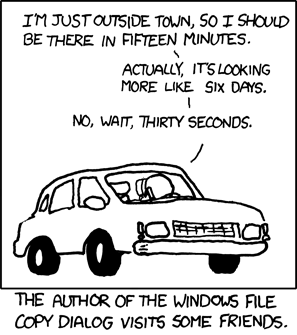
\includegraphics{xkcd-estimation.png} \end{figure}}
      \end{column}
    \end{columns}
  \end{block}


\end{frame}

\begin{frame}
  \frametitle{Reporting VACUUM progress}

  \begin{itemize}
    \item PostgreSQL 10
    \item Add a generic command progress reporting facility.
      \begin{itemize}
	\item \url{http://git.postgresql.org/pg/commitdiff/b6fb6471f6af}
	\item Vinayak Pokale, Rahila Syed, Amit Langote, Robert Haas.
      \end{itemize}
    \item Add simple VACUUM progress reporting.
      \begin{itemize}
	\item \url{http://git.postgresql.org/pg/commitdiff/c16dc1aca5e0}
	\item Amit Langote, Robert Haas, Vinayak Pokale, Rahila Syed.
      \end{itemize}
  \end{itemize}
\end{frame}

\begin{frame}[containsverbatim]
\frametitle{Reporting vacuum progress (2)}
  \footnotesize
\begin{verbatim}
alvherre=# SELECT * FROM pg_stat_progress_vacuum;
\end{verbatim}
\begin{tabular}{c|l}
\multicolumn{2}{c}{\textit{Record 1}} \\
\hline
pid & 4204 \\
datid & 12386 \\
datname & alvherre \\
relid & 234754 \\
phase & scanning heap \\
heap\_blks\_total & 89759 \\
heap\_blks\_scanned & 61181 \\
heap\_blks\_vacuumed & 0 \\
index\_vacuum\_count & 0 \\
max\_dead\_tuples & 291 \\
num\_dead\_tuples & 0 \\
\end{tabular}

\end{frame}

\begin{frame}[fragile]
  \frametitle{Reporting vacuum progress (3)}

  \footnotesize
  \begin{verbatim}
alvherre=# SELECT now(), pid, relid::regclass as table, phase,
           heap_blks_total, heap_blks_scanned, heap_blks_vacuumed,
           index_vacuum_count, max_dead_tuples, num_dead_tuples
           FROM pg_stat_progress_vacuum WHERE datname = current_database();
\end{verbatim}
\begin{tabular}{c|l}
\multicolumn{2}{c}{\textit{Record 1}} \\
\hline
  now & 2019-08-01 11:32:15.300526-04 \\
pid & 4204 \\
table & esquema.tabela \\
phase & scanning heap \\
heap\_blks\_total & 134007 \\
heap\_blks\_scanned & 105442 \\
heap\_blks\_vacuumed & 0 \\
index\_vacuum\_count & 0 \\
max\_dead\_tuples & 291 \\
num\_dead\_tuples & 0 \\
\end{tabular}
\end{frame}

\begin{frame}[fragile]
  \frametitle{Reporting vacuum progress (4)}

  \begin{verbatim}
  alvherre=# \t
  alvherre=# \pset tuples_only on
  alvherre=# SELECT .. FROM pg_stat_progress_vacuum \watch 0,1
  \end{verbatim}

\end{frame}

\begin{frame}
  \frametitle{VACUUM: operation phases}
  \begin{block}{\vspace*{-1cm}}
    \begin{columns}[T]
      \begin{column}{0.55\textwidth}
	\begin{enumerate}
	  \item initializing

	  \item scanning heap

	    \only<2>{ $\rightarrow$ \texttt{dead\_tuples[0 ... maintenance\_work\_mem]} }
	  \item vacuuming indexes
	  \item vacuuming heap
	  \item cleaning up indexes
	  \item truncating heap

	    \only<4->{$\rightarrow$ requires access exclusive lock\\
	    $\rightarrow$ step not done if unavailable}
	  \item performing final cleanup

	    \only<3->{$\rightarrow$ FSM update}
	\end{enumerate}
      \end{column}

      \only<2>{
      \begin{column}{0.35\textwidth}
\begin{tabular}{c|l}
\multicolumn{2}{c}{\textit{Record 1}} \\
\hline
  now & ... \\
pid & ... \\
table & ... \\
phase & ... \\
heap\_blks\_total & 134007 \\
heap\_blks\_scanned & 105442 \\
heap\_blks\_vacuumed & 0 \\
index\_vacuum\_count & 0 \\
max\_dead\_tuples & 291 \\
num\_dead\_tuples & 0 \\
\end{tabular}
      \end{column}
    }
    \end{columns}
  \end{block}

\end{frame}

\begin{frame}
  \frametitle{Reporting CREATE INDEX / REINDEX progress}

  \begin{itemize}
    \item PostgreSQL 12
    \item Report progress of CREATE INDEX operations
      \begin{itemize}
	\item \url{http://git.postgresql.org/pg/commitdiff/ab0dfc961b6a}
	\item Álvaro Herrera
      \end{itemize}
    \item Report progress of REINDEX operations
      \begin{itemize}
	\item \url{http://git.postgresql.org/pg/commitdiff/03f9e5cba0ee}
	\item Peter Eisentraut
      \end{itemize}
  \end{itemize}
\end{frame}

\begin{frame}[fragile]
  \frametitle{Report of CREATE INDEX}

  \footnotesize
  \begin{verbatim}
  SELECT ... FROM pg_stat_progress_create_index ... \watch 1
  \end{verbatim}

\begin{tabular}{c|l}
\hline
pid & 1209 \\
relid & esquema.tabela \\
index\_relid & 35684 \\
command & CREATE INDEX CONCURRENTLY \\
phase & building index: scanning table \\
lockers\_total & 0 \\
lockers\_done & 0 \\
current\_locker\_pid & 0 \\
blocks\_total & 44248 \\
blocks\_done & 17627 \\
tuples\_total & 0 \\
tuples\_done & 0 \\
partitions\_total & 0 \\
partitions\_done & 0 \\
\end{tabular}

\end{frame}

\begin{frame}
  \frametitle{Operation phases of CREATE INDEX / REINDEX}

  \begin{block}{}
    \begin{columns}[T]
      \begin{column}{0.6\textwidth}
	\begin{enumerate}
	  \item initializing
	  \item waiting for writers before build
	  \item building index
	  \item waiting for writers before validation
	  \item index validation: scanning index
	  \item index validation: sorting tuples
	  \item index validation: scanning table
	  \item waiting for old snapshots
	  \item waiting for readers before marking dead
	  \item waiting for readers before dropping
	\end{enumerate}
      \end{column}

      \only<2>{
      \begin{column}{0.35\textwidth}
	\begin{tabular}{c|l}
	  \hline
	  phase & .... \\
	  lockers\_total & 0 \\
	  lockers\_done & 0 \\
	  current\_locker\_pid & 0 \\
	  blocks\_total & 44248 \\
	  blocks\_done & 17627 \\
	  tuples\_total & 0 \\
	  tuples\_done & 0 \\
	  partitions\_total & 0 \\
	  partitions\_done & 0 \\
	\end{tabular}
      \end{column}
    }
    \end{columns}
  \end{block}
\end{frame}

\begin{frame}
  \frametitle{Build phases for B-Tree indexes}
  \begin{enumerate}
    \item initializing
    \item scanning table
    \item sorting live tuples
    \item sorting dead tuples
    \item loading tuples in tree
  \end{enumerate}
\end{frame}

\begin{frame}
  \frametitle{Reporting CLUSTER / VACUUM FULL progress}

  \begin{itemize}
    \item PostgreSQL 12
    \item Add progress reporting for CLUSTER and VACUUM FULL.
      \begin{itemize}
	\item \url{http://git.postgresql.org/pg/commitdiff/6f97457e0ddd}
	\item Tatsuro Yamada
      \end{itemize}
  \end{itemize}

\end{frame}

\begin{frame}[fragile]
   \frametitle{Reporting cluster progress}

\footnotesize
\begin{verbatim}
alvherre=# SELECT * FROM pg_stat_progress_cluster \watch 1
\end{verbatim}

\noindent 
\begin{tabular}{c|l}
\hline
pid & 1209 \\
table & esquema.tabela \\
command & VACUUM FULL \\
phase & seq scanning heap \\
cluster\_index\_relid & 0 \\
heap\_tuples\_scanned & 8064358 \\
heap\_tuples\_written & 8064358 \\
heap\_blks\_total & 44248 \\
heap\_blks\_scanned & 35684 \\
index\_rebuild\_count & 0 \\
\end{tabular}
\end{frame}

\begin{frame}
  \frametitle{CLUSTER: operation phases}

  \begin{enumerate}
    \item initializing
    \item seq scanning heap
    \item index scanning heap
    \item sorting tuples
    \item writing new heap
    \item swapping relation files
    \item rebuilding index
    \item performing final cleanup
  \end{enumerate}
\end{frame}

\begin{frame}
  \frametitle{Reporting ANALYZE progress}

  \begin{itemize}
    \item Patch submitted for PostgreSQL 13
    \item \url{https://postgr.es/m/20190621185207.GA27929@alvherre.pgsql}
  \end{itemize}
\end{frame}

\begin{frame}
  \frametitle{Questions?}

  \centering
  Thanks for listening!

\end{frame}

\begin{frame}[fragile]
  \frametitle{Appendix: Implementation}

  \begin{itemize}
    \item Set-returning function \texttt{pg\_stat\_get\_progress\_info(text)}
    \item Returns raw metrics
    \item View definitions (\texttt{pg\_stat\_progress\_vacuum} etc) transform metrics
      into user-readable parameters
    \item PostgreSQL C code injects metrics into \texttt{pgstat} system
  \end{itemize}
\vfill
\begin{verbatim}
pgstat_progress_start_command(command type);
pgstat_progress_update_param(4, 158);
pgstat_progress_update_param(PROGRESS_ANALYZE_PHASE,
                             PROGRESS_ANALYZE_PHASE_SCAN_TABLE);
pgstat_progress_end_command();
  \end{verbatim}

\end{frame}

\end{document}
